\section{Example Application: Fuzzy Extension Principle}
\label{sec:55fuzzy}

\minitoc[-1mm]{84mm}{4}

\noindent
To conclude this chapter, we consider the fuzzy extension principle
as an example application of optimization of B-spline sparse grid surrogates.

\paragraph{Aleatoric and epistemic uncertainties}

Classical uncertainty quantification (UQ) distinguishes between
aleatoric and epistemic uncertainties \cite{Walz16Fuzzy}.
Aleatoric uncertainties result from the variability of inputs or
model components and from the ``intrinsic randomness''
of quantities.
They are best described by probability theory, giving exact probabilities.
Epistemic uncertainties arise from subjectivity,
simplifying modeling assumptions, and incomplete knowledge.
These uncertainties are better captured by fuzzy theory,
which is more imprecise than the ``exact'' stochastic assumptions
of probabilities \cite{Walz16Fuzzy}.

\paragraph{Uncertainty quantification with fuzzy uncertainties}

In uncertainty quantification, the key question is as follows:
Given a model and uncertain input parameters for the model,
how uncertain is the model output?
While there are many approaches available
for probabilistic uncertainties,
it is not straightforward to solve this task
for fuzzy uncertainties.
Fortunately, Zadeh proposed in 1975
the \term{fuzzy extension principle} \cite{Zadeh75Concept},
which addresses this very question.

\paragraph{Sparse grids and B-splines for fuzzy uncertainties}

As we explain in this section,
the fuzzy extension principle requires the solution of numerous
optimization problems that involve the original objective function
$\objfun$.
This predestines the replacement of $\objfun$ with sparse grid surrogates,
as explained in the beginning of the chapter.
Previous work by Klimke \cite{Klimke06Uncertainty} already
studied this approach for piecewise linear functions on uniform sparse grids
and for global polynomials on sparse Clenshaw--Curtis grids.
We assess the suitability of interpolation with higher-order
hierarchical B-splines on sparse grids for the fuzzy extension principle.
It should be mentioned that there is also work
directly incorporating (non-hierarchical) B-splines
into the framework of fuzzy theory for modeling uncertain surfaces
\multicite{Anile00Modeling,Zakaria14Fuzzy}.



\subsection{Fuzzy Sets and Fuzzy Intervals}
\label{sec:551fuzzySets}

In the following, we repeat very briefly the necessary
definitions of basic fuzzy theory.
Examples for the definitions are shown in \cref{fig:fuzzySet}.
A more in-depth introduction can be found in
\multicite{Hanss05Applied,Klimke06Uncertainty,Walz16Fuzzy}.

\begin{figure}
  \subcaptionbox{%
    Non-convex fuzzy set \emph{\textcolor{C0}{(blue)}}
    and $\alpha$-cut \emph{\textcolor{C1}{(red)}.}%
  }[46mm]{%
    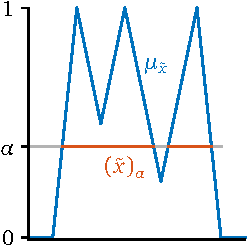
\includegraphics{fuzzySet_1}%
  }%
  \hfill%
  \subcaptionbox{%
    Fuzzy interval.%
  }[43mm]{%
    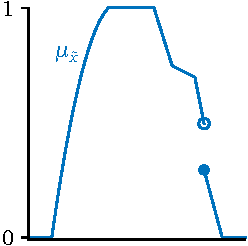
\includegraphics{fuzzySet_2}%
  }%
  \hfill%
  \subcaptionbox{%
    Common types of fuzzy numbers and intervals (see text).%
  }[56mm]{%
    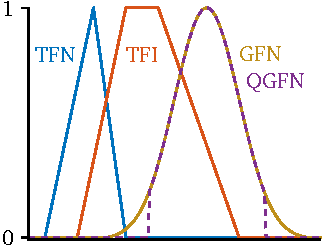
\includegraphics{fuzzySet_3}%
  }%
  \caption[%
    Examples of fuzzy sets and $\alpha$-cuts%
  ]{%
    Examples of membership functions of fuzzy sets and $\alpha$-cuts.%
  }%
  \label{fig:fuzzySet}%
\end{figure}

\paragraph{Fuzzy sets}

Let $X \subset \real$ be a closed interval on the real line
and $\memfun{x}\colon X \to \clint{0, 1}$ be a function.
We call the graph $\fuzzy{x} \ceq \{(x, \memfun{x}(x) \mid x \in X\}$
of $\memfun{x}$ a \term{fuzzy set} with
\term{membership function} $\memfun{x}$.
Fuzzy sets generalize ordinary subsets of $X$,
which can be obtained by requiring $\memfun{x}(X) \subset \{0, 1\}$.
In this case, the fuzzy set is called \term{crisp} and
$\fuzzy{x}$ can be identified with the ordinary set
$\{x \in X \mid \memfun{x}(x) = 1\}$.
A fuzzy set $\fuzzy{x}$ is \term{normalized}
if $\max_{x \in X} \memfun{x}(x) = 1$.
A \term{convex} fuzzy set $\fuzzy{x}$ satisfies
$\min(\memfun{x}(a), \memfun{x}(c)) \le \memfun{x}(b)$ for all $a, b, c \in X$
with $a \le b \le c$.

\paragraph{Fuzzy intervals and $\alpha$-cuts}

A convex and normalized fuzzy set $\fuzzy{x}$ with
piecewise continuous membership function $\memfun{x}$ is called
\term{fuzzy interval.}
If $\{x \in X \mid \memfun{x}(x) = 1\} = \{a\}$ for some $a \in X$,
then the fuzzy interval $\fuzzy{x}$ is called \term{fuzzy number.}

For $\alpha \in \clint{0, 1}$, the $\alpha$-cut of $\fuzzy{x}$ is
defined as $\acut{x}{\alpha} \ceq \{x \in X \mid \memfun{x}(x) \ge \alpha\}$
for $\alpha > 0$ and $\acut{x}{0} \ceq \supp \memfun{x}$ for $\alpha = 0$.
The $\alpha$-cuts of fuzzy intervals $\fuzzy{x}$ are always
nested closed intervals, i.e.,
$\acut{x}{\alpha} = [a, b]$ for some $a \le b$ and
$\acut{x}{\alpha_1} \supset \acut{x}{\alpha_2}$ for $\alpha_1 \le \alpha_2$.

\paragraph{Common types of fuzzy numbers and intervals}

There are various types of fuzzy numbers and intervals
\cite{Klimke06Uncertainty}.
Most common are
\term{triangular fuzzy numbers} (TFNs, i.e., linear B-splines),
\term{trapezoidal fuzzy intervals}
(TFIs, where a plateau of height one is inserted at the peak, i.e.,
sums of two neighboring linear B-splines), and
\term{Gaussian fuzzy numbers} (GFNs) with membership function
$\memfun{x}(x) = \exp(-\frac{(x - \mu)^2}{(2\sigma)^2})$.
As the support of Gaussian fuzzy numbers is unbounded,
\term{quasi-Gaussian fuzzy numbers} (QGFNs) truncate the support
to a fixed multiple of the standard deviation $\sigma$
\cite{Klimke06Uncertainty}.
However, it would be more natural to directly employ B-splines of
degree $p > 1$ (normalized adequately), since they generalize
triangular fuzzy numbers and their limit with respect to $p$
is a Gaussian fuzzy number.



\subsection{Fuzzy Extension Principle}
\label{sec:552fuzzyExtensionPrinciple}

Let $\objfun\colon \clint{\*0, \*1} \to \real$ be an objective function,
whose values $y = \objfun(\*x)$ represent the results of the
simulation of a model with input parameters $(x_1, \dotsc, x_d) = \*x$.
If the input parameters are uncertain and
given as fuzzy sets $\fuzzy{x}_1, \dotsc, \fuzzy{x}_d$,
what is the resulting uncertain outcome
``$\fuzzy{y} \ceq \objfun(\fuzzy{x}_1, \dotsc, \fuzzy{x}_d)$''?
Note that there is no definite answer to this question,
as ``$\objfun(\fuzzy{x}_1, \dotsc, \fuzzy{x}_d)$'' is not well-defined.
The fuzzy extension principle, suggested by Zadeh \cite{Zadeh75Concept},
provides one possible definition.

\paragraph{Alternative fuzzy extension principle}

We use an alternative formulation of the fuzzy extension principle,
which is stated in \cite{Klimke06Uncertainty}.
The original formulation is computationally more complex,
as it requires the solution of equality-constrained optimization problems
and one needs to know the range of $\objfun$, which might not be given.
The two formulations are equivalent,
if $\fuzzy{x}_1, \dotsc, \fuzzy{x}_d$ are (compactly supported)
fuzzy intervals and $\objfun$ is continuous \cite{Buckley90Using},
which we assume in the following.

The alternative fuzzy extension principle defines
``$\fuzzy{y} = \objfun(\fuzzy{x}_1, \dotsc, \fuzzy{x}_d)$'' as the fuzzy set
$\fuzzy{y}$ with
\begin{subequations}
  \label{eq:alternativeFuzzyExtensionPrinciple}
  \begin{alignat}{2}
    \memfun{y}(y)
    &\ceq \sup\{\alpha \in \clint{0, 1} \mid y \in \acut{y}{\alpha}\},\quad
    &&y \in \real,\\
    \acut{y}{\alpha}
    &\ceq \bracket*{
      \min_{\*x \in \Omega_\alpha} \objfun(\*x),\;
      \max_{\*x \in \Omega_\alpha} \objfun(\*x)
    },\quad
    &&\alpha \in \clint{0, 1},\\
    \Omega_\alpha
    &\ceq \acut[1]{x}{\alpha} \times \dotsb \times \acut[d]{x}{\alpha},\quad
    &&\alpha \in \clint{0, 1}.
  \end{alignat}
\end{subequations}
This definition is visualized in \cref{fig:fuzzyExtensionPrinciple}.
The first equation defines $\fuzzy{y}$ via its $\alpha$-cuts,
which are given in the second equation as the closed interval
between the minimal and the maximal value of $\objfun$ on some
hyper-rectangular domain $\Omega_\alpha$.
The third equation specifies this domain $\Omega_\alpha$ as the
Cartesian product of the univariate $\alpha$-cuts.
Hence, we only have to solve box-constrained optimization problems,
as opposed to the general equality-constrained problems
in the original formulation of the fuzzy extension principle.

\begin{figure}
  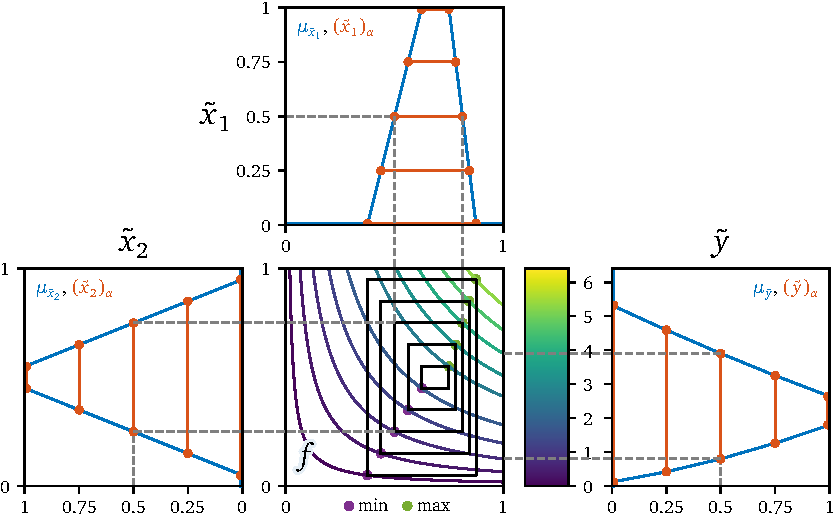
\includegraphics{fuzzyExtensionPrinciple_1}%
  \caption[%
    Alternative fuzzy extension principle%
  ]{%
    Example of the application of the
    alternative fuzzy extension principle to the bivariate objective function
    $\objfun(\*x) = 6.4 x_1 x_2$ \emph{(bottom)}
    and triangular fuzzy input intervals
    $\fuzzy{x}_1$ and $\fuzzy{x}_2$ \emph{(top and left)}
    to obtain the fuzzy output interval $\fuzzy{y}$ \emph{(right).}
    Adapted from \cite{Klimke06Uncertainty}.%
  }%
  \label{fig:fuzzyExtensionPrinciple}%
\end{figure}

\paragraph{Implementation}

The implementation of the alternative fuzzy extension principle
is straightforward and shown in \cref{alg:alternativeFuzzyExtensionPrinciple}
\cite{Klimke06Uncertainty}.
The range $\clint{0, 1}$ of $\alpha$
is discretized into $m + 1$ uniformly spaced values $\alpha_j$
(where $m \in \nat$).
For each of these values $\alpha_j$, we compute the corresponding
$\alpha_j$-cut of $\fuzzy{y}$ by solving the two box-constrained
optimization problems of \cref{eq:alternativeFuzzyExtensionPrinciple}.
The fuzzy output interval $\fuzzy{y}$ can then be approximated by
interpolating the interval bounds of the $\alpha_j$-cuts of $\fuzzy{y}$.

\begin{algorithm}
  \begin{algorithmic}[1]
    \Function{$\fuzzy{y} = \texttt{alternativeFuzzyExtensionPrinciple}$}{%
      $m$, $\fuzzy{x}_1$, \dots, $\fuzzy{x}_d$%
    }
      \For{$j = 0, \dotsc, m$}
        \State{$\alpha_j \gets j/m$}
        \ForOneLine{$t = 1, \dotsc, d$}{Compute $\acut[t]{x}{\alpha_j} = \clint{a_{j,t}, b_{j,t}}$}
        \State{%
          $\Omega_{\alpha_j} \gets \acut[1]{x}{\alpha_j} \times \dotsb \times
          \acut[d]{x}{\alpha_j} = \clint{\*a_j, \*b_j}$%
        }
        \State{%
          Solve $\min_{\*x \in \Omega_{\alpha_j}} \objfun(\*x)$ and
          $\max_{\*x \in \Omega_{\alpha_j}} \objfun(\*x)$%
        }
        \State{%
          $\acut{y}{\alpha_j} = [c_j, d_j] \gets \clint{
            \min_{\*x \in \Omega_{\alpha_j}} \objfun(\*x),
            \max_{\*x \in \Omega_{\alpha_j}} \objfun(\*x)
          }$
        }
      \EndFor{}\vspace{-2mm}
      \State{%
        $D \gets
        \{(c_j, \alpha_j) \mid j = 0,\, 1,\, \dotsc,\, m\} \cup
        \{(d_j, \alpha_j) \mid j = m,\, m - 1,\, \dotsc,\, 0\}$%
      }
      \State{%
        $\memfun{y} \gets \text{Piecewise linear interpolant of $D$}$%
      }%
      \Comment{extend to $X$ by zero}%
    \EndFunction{}
  \end{algorithmic}
  \caption[Alternative fuzzy extension principle]{%
    Alternative fuzzy extension principle.
    Inputs are the number of $\alpha$ segments to use as discretization and
    the $d$ fuzzy intervals $\fuzzy{x}_1, \dotsc, \fuzzy{x}_d$
    (we have to be able to determine $\alpha$-cuts
    of these fuzzy input intervals).
    The output is an approximation to the output $\fuzzy{y}$
    of the alternative fuzzy extension principle
    (given by an approximation of its membership function $\memfun{y}$).%
  }%
  \label{alg:alternativeFuzzyExtensionPrinciple}%
\end{algorithm}



\subsection{Using B-Splines on Sparse Grids to Propagate Fuzzy Uncertainties}
\label{sec:553fuzzyBSplines}

Following Klimke's approach \cite{Klimke06Uncertainty},
we replace the objective function $\objfun$ in
\cref{alg:alternativeFuzzyExtensionPrinciple}
with a sparse grid surrogate $\sgintp$.
The solution of the optimization problems
$\min_{\*x \in \Omega_{\alpha_j}} \sgintp(\*x)$ and
$\max_{\*x \in \Omega_{\alpha_j}} \sgintp(\*x)$ with respect to the
surrogate $\sgintp$ instead of the true objective function $\objfun$
takes significantly less time, if evaluations of the objective function
are expensive.

However, Klimke used piecewise linear functions as the hierarchical basis on
uniform sparse grids and global polynomials on sparse Clenshaw--Curtis grids.
The drawbacks of each of the bases are evident:
First, piecewise linear surrogates are not continuously differentiable and
can thus not be optimized well with gradient-based optimization methods.
Second, global polynomials are only suitable for
Clenshaw--Curtis grids (Chebyshev-distributed points)
due to Runge's phenomenon,
unnecessarily restricting the choice of grid points.
Hierarchical B-splines of degree $p$ are $(p - 1)$ times
continuously differentiable and defined for arbitrary point
distributions, eliminating both drawbacks simultaneously.

\paragraph{Methodology}

Given a sparse grid $\sgset$, which may be regular or spatially adaptive,
we compute three solutions of the alternative fuzzy extension principle
as follows:

\begin{itemize}
  \item
  First,
  we replace $\objfun$ in \cref{alg:alternativeFuzzyExtensionPrinciple}
  with the sparse grid interpolant $\sgintp[p]$
  on $\sgset$ using modified hierarchical not-a-knot B-splines
  $\bspl[\nak,\modified]{l,i}{p}$ of cubic degree ($p = 3$).
  For solving the optimization problems over $\sgintp[p]$ in
  \cref{alg:alternativeFuzzyExtensionPrinciple},
  we use the globalized version of the method of gradient descent
  as described in \cref{sec:522method} using 100 initial points.
  The resulting fuzzy output interval is denoted by $\fuzzy[\sparse,p]{y}$.
  
  \item
  Second,
  we replace $\objfun$ in \cref{alg:alternativeFuzzyExtensionPrinciple}
  with the sparse grid interpolant $\sgintp[1]$
  on $\sgset$ using modified piecewise linear basis functions.
  For solving the optimization problems over $\sgintp[1]$ in
  \cref{alg:alternativeFuzzyExtensionPrinciple},
  we use a multi-start version of the Nelder--Mead method
  as described in \cref{sec:522method}
  using 100 initial simplices%
  \footnote{%
    The Nelder--Mead method does not require an initial point,
    but an initial simplex.
    The method is a hybrid between global and local optimization.
    If the initial simplex is chosen badly, Nelder--Mead may get stuck
    in local minima.
    Hence, we restart the algorithm for different initial simplices.%
  }.
  The resulting fuzzy output interval corresponds to Klimke's method and
  is denoted by $\fuzzy[\sparse,1]{y}$.
  
  \item
  Third,
  for comparison, we solve
  \cref{alg:alternativeFuzzyExtensionPrinciple} for the
  actual objective function $\objfun$.
  For solving the optimization problems over $\objfun$,
  we use a multi-start version of the Nelder--Mead method
  as described in \cref{sec:522method}
  using 1000 initial simplices
  and \num{2000000} allowed evaluations of $\objfun$.
  The resulting fuzzy output interval is denoted by $\fuzzy[\reference]{y}$
  \term{(reference solution).}
\end{itemize}

\noindent
In the following, we fix the number of $\alpha$ segments
in \cref{alg:alternativeFuzzyExtensionPrinciple} as $m = 100$.
As fuzzy input intervals $\fuzzy{x}_t$, $t = 1, \dotsc, d$, we use
the trapezoidal fuzzy interval with $0$-cut $\clint{0.125, 0.625}$
and $1$-cut $\clint{0.25, 0.375}$ if $t$ is odd and
the quasi-Gaussian fuzzy number with mean $0.5$, standard deviation $0.125$,
and $0$-cut $\clint{0.125, 0.875}$ if $t$ is even.

\paragraph{Convergence of fuzzy intervals on regular sparse grids}

As an example,
\cref{fig:resultsFuzzyPropagation} shows the convergence of the
fuzzy output intervals $\fuzzy[\sparse,p]{y}$ and $\fuzzy[\sparse,1]{y}$
obtained by the interpolation of the
bivariate Alp02 function on regular sparse grids $\sgset = \regsgset{n}{d}$
to the reference solution $\fuzzy[\reference]{y}$.
Already for $n = 4$, the B-spline approximation is better than the
piecewise linear approximation.
For $n = 5$, no difference is visible anymore between $\fuzzy[\sparse,p]{y}$
and $\fuzzy[\reference]{y}$, while $\fuzzy[\sparse,1]{y}$ still clearly
deviates from $\fuzzy[\reference]{y}$.

\begin{SCfigure}
  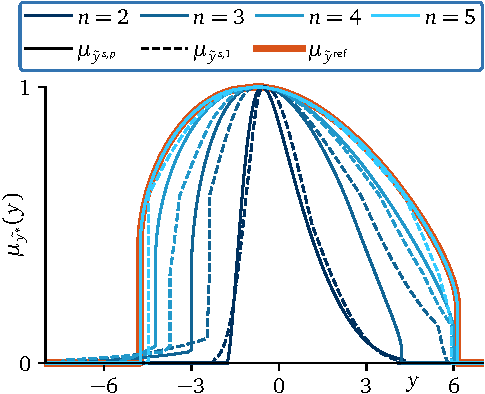
\includegraphics{resultsFuzzyPropagation_1}%
  \caption[Convergence of fuzzy output intervals]{%
    Convergence of the membership functions of the fuzzy output intervals
    $\fuzzy[\sparse,p]{y}$
    (\emph{solid lines,} modified hierarchical cubic not-a-knot B-splines)
    and $\fuzzy[\sparse,1]{y}$
    (\emph{dashed,} modified hierarchical hat functions)
    to the reference solution $\fuzzy[\reference]{y}$
    \emph{\textcolor{C1}{(red)}} for the bivariate Alp02 function using
    regular sparse grids of level $n = 2, \dotsc, 5$.%
  }%
  \label{fig:resultsFuzzyPropagation}%
\end{SCfigure}

In \cref{fig:resultsFuzzyRegular}, we study the convergence of the
relative $\Ltwo$ errors
\begin{equation}
  e^{\sparse,\ast}
  \ceq \frac{
    \normLtwo{\memfun[\reference]{y} - \memfun[\sparse,\ast]{y}}
  }{
    \normLtwo{\memfun[\reference]{y}}
  },\quad
  \ast \in \{1, p\},
\end{equation}
of the membership functions (``fuzzy errors'').
The Alp02 ($d = 2$) errors
that correspond to \cref{fig:resultsFuzzyPropagation}
are shown in green in the left-most plot of \cref{fig:resultsFuzzyRegular}.
For the Bra02, GoP\punctfix{,} and Alp02 functions,
B-spline surrogates achieve
dramatic improvements over the hat function surrogates in the bivariate case.
For the bivariate Ack function, B-splines yield an error that
is still an order of magnitude smaller than the error of hat functions.
Just little or even no improvement can be seen
for the functions Sch06 and Sch22 with discontinuous derivatives or
higher dimensionalities $d \ge 4$.

\begin{figure}
  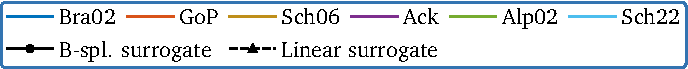
\includegraphics{resultsFuzzyLegend_1}\\[2mm]%
  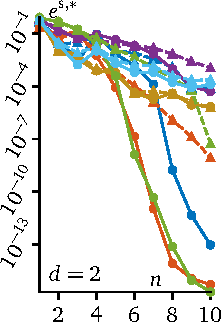
\includegraphics{resultsFuzzyRegular_1}%
  \hfill%
  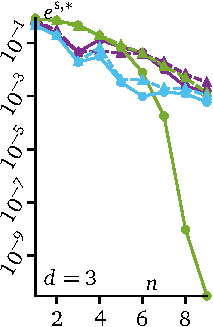
\includegraphics{resultsFuzzyRegular_2}%
  \hfill%
  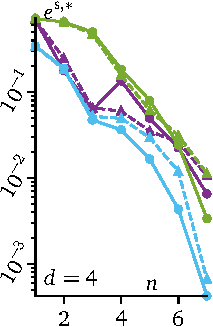
\includegraphics{resultsFuzzyRegular_3}%
  \hfill%
  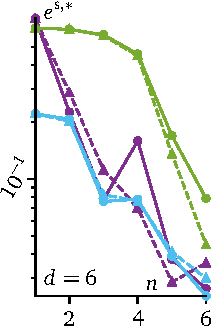
\includegraphics{resultsFuzzyRegular_4}%
  \caption[Fuzzy errors for regular sparse grids]{%
    Fuzzy errors
    $e^{\sparse,\ast}
    \ceq \normLtwo{\memfun[\reference]{y} - \memfun[\sparse,\ast]{y}}/
    \normLtwo{\memfun[\reference]{y}}$
    for regular sparse grids $\regsgset{n}{d}$
    and different objective functions $\objfun$ \emph{(colors)}
    over the level $n$ of the sparse grid.%
  }%
  \label{fig:resultsFuzzyRegular}%
\end{figure}

\paragraph{Fuzzy Novak--Ritter method}

We want to employ spatial adaptivity to improve the results
of regular sparse grids.
To this end, we modify the Novak--Ritter criterion
to create a grid generation method that is tailored for the
fuzzy extension principle, resulting in \cref{alg:fuzzyNovakRitterMethod}.
Its main idea is to generate more points near the optima
of the fuzzy extension principle
(\cref{alg:alternativeFuzzyExtensionPrinciple}) than in other regions
of $\clint{\*0, \*1}$.
Therefore, we apply the Novak--Ritter criterion twice to
every $\alpha$ level $\alpha_j = \tfrac{j}{m}$ ($j = 0, \dotsc, m$),
once for the minimum and once for the maximum.
For all $\alpha_j$, the points to be refined are collected in a set.
If a point is selected multiple times for different $\alpha_j$,
it is refined only once.
In addition, we enlarge the search domain $\Omega_{\alpha_j}$
by \SI{10}{\percent}, since the minimum or the maximum might be
near the boundary $\Omega_{\alpha_j}$ and
since the points to be inserted might not be close to
the points to be refined.
We ensure that the size of $\Omega_{\alpha_j}$ is at least $0.05$
in every coordinate direction.
The remaining experiments use $\gamma = 0.1$ as adaptivity.

\begin{algorithm}
  \begin{algorithmic}[1]
    \Function{$\liset = \texttt{fuzzyNovakRitterMethod}$}{%
      $\objfun$, $\gamma$, $m$, $\liset$, $\fuzzy{x}_1$, \dots, $\fuzzy{x}_d$%
    }
      \ForOneLine{$(\*l, \*i) \in \liset$}{$d_{\*l,\*i} \gets 0$}
      \Comment{degrees (number of refinements)}%
      \While{$\setsize{\liset} < \ngpMax$}
        \State{$R \gets \emptyset$}
        \For{$j = 0, \dotsc, m$}
          \State{$\alpha_j \gets j/m$}
          \For{$t = 1, \dotsc, d$}
            \State{$\clint{a_{j,t}, b_{j,t}} \gets \acut[t]{x}{\alpha_j}$}
            \Comment{determine $\alpha_j$-cut}%
            \If{$b_{j,t} - a_{j,t} < 0.05$}
            \Comment{ensure minimal size of $0.05$}%
              \State{%
                $(a_{j,t}, b_{j,t}) \gets
                ((a_{j,t} + b_{j,t})/2 - 0.025,
                (a_{j,t} + b_{j,t})/2 + 0.025)$%
              }\vspace{-1mm}
            \EndIf{}
            \State{%
              $(a_{j,t}, b_{j,t}) \gets
              (a_{j,t} - 0.05 (b_{j,t} - a_{j,t}),
              b_{j,t} + 0.05 (b_{j,t} - a_{j,t}))$%
            }
            \Comment{enlarge by \SI{10}{\percent}}%
            \vspace{-1mm}
          \EndFor{}
          \State{%
            $\liset_j \gets \{(\*l, \*i) \in \liset \mid
            \gp{\*l,\*i} \in \clint{\*a_j, \*b_j} \cap \clint{\*0, \*1}\}$%
          }
          \Comment{%
            set of feasible points
            ($\clint{\*a_j, \*b_j} = \Omega_{\alpha_j}$)%
          }%
          \ForOneLine{$(\*l, \*i) \in \liset_j$}{%
            $r_{\*l,\*i} \gets \setsize{
              \{(\*l', \*i') \in \liset_j \mid
              \objfun(\gp{\*l',\*i'}) \le \objfun(\gp{\*l,\*i})\}
            }$%
          }
          \Comment{ranks}%
          \State{%
            $(\*l^\ast, \*i^\ast) \gets
            \vecargmin_{(\*l,\*i) \in \liset_j} \bracket*{
              (r_{\*l,\*i} + 1)^\gamma
              (\normone{\*l} + d_{\*l,\*i} + 1)^{1 - \gamma}
            }$%
          }
          \Comment{for minimum}%
          \vspace{-0.7mm}
          \State{%
            $(\*l^{\ast\ast}, \*i^{\ast\ast}) \gets
            \vecargmin_{(\*l,\*i) \in \liset_j} \bracket*{
              (\setsize{\liset_j} - r_{\*l,\*i} + 2)^\gamma
              (\normone{\*l} + d_{\*l,\*i} + 1)^{1 - \gamma}
            }$%
          }
          \Comment{for maximum}%
          \State{%
            $R \gets R \cup \{(\*l^\ast, \*i^\ast),
            (\*l^{\ast\ast}, \*i^{\ast\ast})\}$%
          }
        \EndFor{}
        \State{Refine all points in $\liset$ that are in $R$}
        \ForOneLine{$(\*l, \*i) \in R$}{$d_{\*l,\*i} \gets d_{\*l,\*i} + 1$}
      \EndWhile{}
    \EndFunction{}
  \end{algorithmic}
  \caption[Fuzzy Novak--Ritter method]{%
    Fuzzy Novak--Ritter method to generate spatially adaptive sparse grids
    for the fuzzy extension principle.
    Inputs are
    the objective function $\objfun$,
    the adaptivity parameter $\gamma \in \clint{0, 1}$,
    the number of $\alpha$ segments,
    the initial sparse grid $\liset$ as a set of level-index pairs, and
    the $d$ fuzzy intervals $\fuzzy{x}_1, \dotsc, \fuzzy{x}_d$.
    The output is the spatially adaptive sparse grid $\liset$.%
  }%
  \label{alg:fuzzyNovakRitterMethod}%
\end{algorithm}

\paragraph{Convergence of fuzzy intervals on spatially adaptive sparse grids}

As we can see in \cref{fig:resultsFuzzyAdaptive},
the spatially adaptive sparse grids generated by the fuzzy Novak--Ritter
method improve results significantly
for both cubic B-spline and piecewise linear surrogates.
However, the performance of the B-spline surrogates benefits more
from the spatial adaptivity.
Even for higher-dimensional settings such as $d = 6$,
the spatial adaptivity helps to decrease the errors by one order of magnitude.
For instance, for the Ack function in six variables,
we can achieve an error of \SI{2.6}{\percent}
with a budget of \num{10000} objective function evaluations (grid points)
on regular sparse grids.
With the same budget and with spatial adaptivity, the error drops below
\SI{0.25}{\percent}.
Conversely, to achieve the same error as in the regular case
(\SI{2.6}{\percent}),
only \SI{1600} evaluations are needed for spatially adaptive grids.

\begin{figure}
  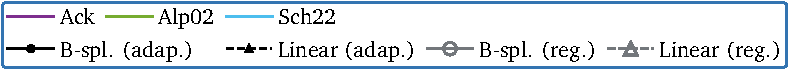
\includegraphics{resultsFuzzyLegend_2}\\[2mm]%
  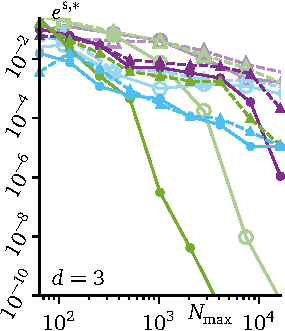
\includegraphics{resultsFuzzyAdaptive_1}%
  \hfill%
  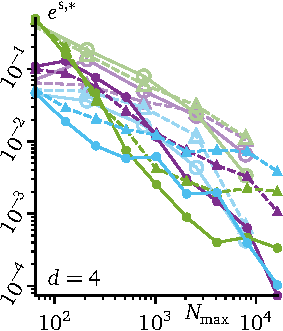
\includegraphics{resultsFuzzyAdaptive_2}%
  \hfill%
  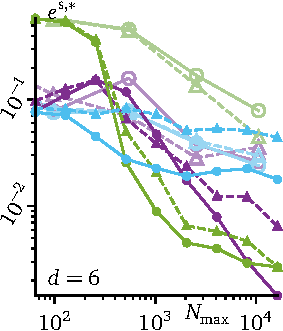
\includegraphics{resultsFuzzyAdaptive_3}%
  \caption[Fuzzy errors for spatially adaptive sparse grids]{%
    Fuzzy errors
    $e^{\sparse,\ast}
    \ceq \normLtwo{\memfun[\reference]{y} - \memfun[\sparse,\ast]{y}}/
    \normLtwo{\memfun[\reference]{y}}$
    for spatially adaptive sparse grids $\sgset$ \emph{(solid markers)}
    and different objective functions $\objfun$ \emph{(colors)}
    over the number $\ngpMax$ of objective function evaluations.
    For comparison, the results of \cref{fig:resultsFuzzyRegular}
    for regular sparse grids are repeated \emph{(hollow markers).}%
  }%
  \label{fig:resultsFuzzyAdaptive}%
\end{figure}
